\section*{Problema 1}
\textbf{Implementa y evalúa las siguientes integrales usando la regla compuesta de Simpson 3/8 para n=\{3,6,9,12,15\} y muestra una gráfica de n contra el valor absoluto del error.}

\begin{enumerate}
    \item \begin{equation*}
              \int_{-1}^1 e^x dx
          \end{equation*}
          \begin{table}[H]
              \centering
              \begin{tabular}{ccc} \hline
                  \textbf{Puntos} & \textbf{Resultado} & \textbf{Diferencia} \\ \hline
                  3               & 2.355648           & 0.005246            \\
                  6               & 2.350756           & 0.000354            \\
                  9               & 2.350473           & 0.000071            \\
                  12              & 2.350425           & 0.000023            \\
                  15              & 2.350412           & 0.000010            \\ \hline
              \end{tabular}
          \end{table}

          \begin{figure}[H]
              \centering
              \begin{subfigure}[b]{8cm}
                  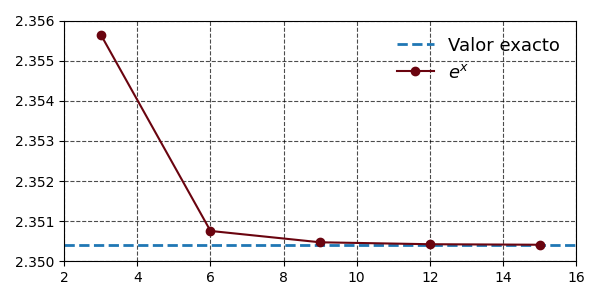
\includegraphics[width=8cm]{Graphics/problema01_fun_f1.png}
                  \caption{}
              \end{subfigure}
              \begin{subfigure}[b]{8cm}
                  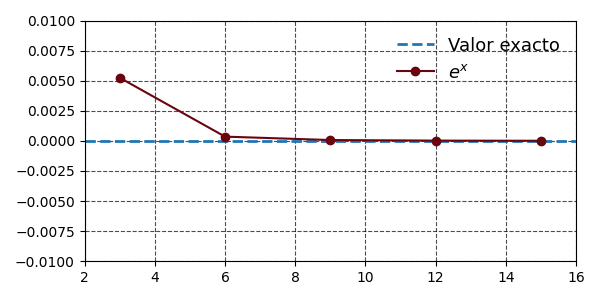
\includegraphics[width=8cm]{Graphics/problema01_diff_f1.png}
                  \caption{}
              \end{subfigure}
              \caption{}
          \end{figure}
    \item \begin{equation*}
              \int_{-1}^{1} \frac{1}{x^2+1} dx
          \end{equation*}

          \begin{table}[H]
              \centering
              \begin{tabular}{ccc} \hline
                  \textbf{Puntos} & \textbf{Resultado} & \textbf{Diferencia} \\ \hline
                  3               & 1.600000           & 2.920367e-02        \\
                  6               & 1.569231           & 1.565327e-03        \\
                  9               & 1.570850           & 5.367321e-05        \\
                  12              & 1.570792           & 4.326795e-06        \\
                  15              & 1.570796           & 3.267949e-07        \\ \hline
              \end{tabular}
          \end{table}

          \begin{figure}[H]
              \centering
              \begin{subfigure}[b]{8cm}
                  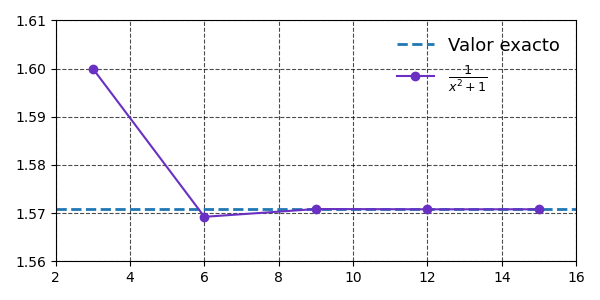
\includegraphics[width=8cm]{Graphics/problema01_fun_f2.png}
                  \caption{}
              \end{subfigure}
              \begin{subfigure}[b]{8cm}
                  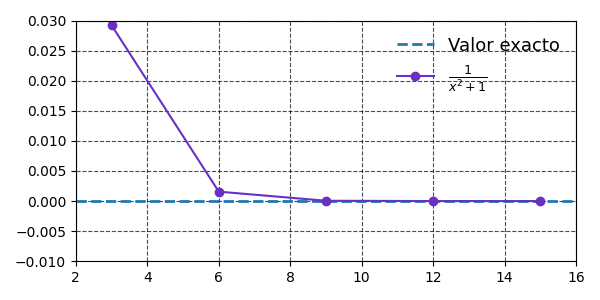
\includegraphics[width=8cm]{Graphics/problema01_diff_f2.png}
                  \caption{}
              \end{subfigure}
              \caption{}
          \end{figure}
\end{enumerate}

